\documentclass[../main.tex]{subfiles}
\begin{document}
\section{Introduction}\label{sec:Introduction}
This project is based on preliminary notes the author wrote a few years ago 
about concrete examples and counterexamples, constructions and computations in elementary algebraic geometry.

The goal of the notes is to serve as some kind of complimentary materials for people who want
to start learning algebraic geometry. Besides theorems and lemmas in classical textbooks,
people can have concrete objects to get hands dirty. 

The notes is still in a rough form, the essentials are there, errors are floating around as well. 
Use it in a dialectical way and you're sincerely welcomed to modify/correct/add materials in the \href{https://github.com/Waerden001/Examples-and-Counterexamples-in-Elementary-Algebraic-Geometry}{GitHub repository for this project}. 

By downloading the file, you solemnly swear to send me any mistakes you find.
\begin{figure}[h!]
\centering
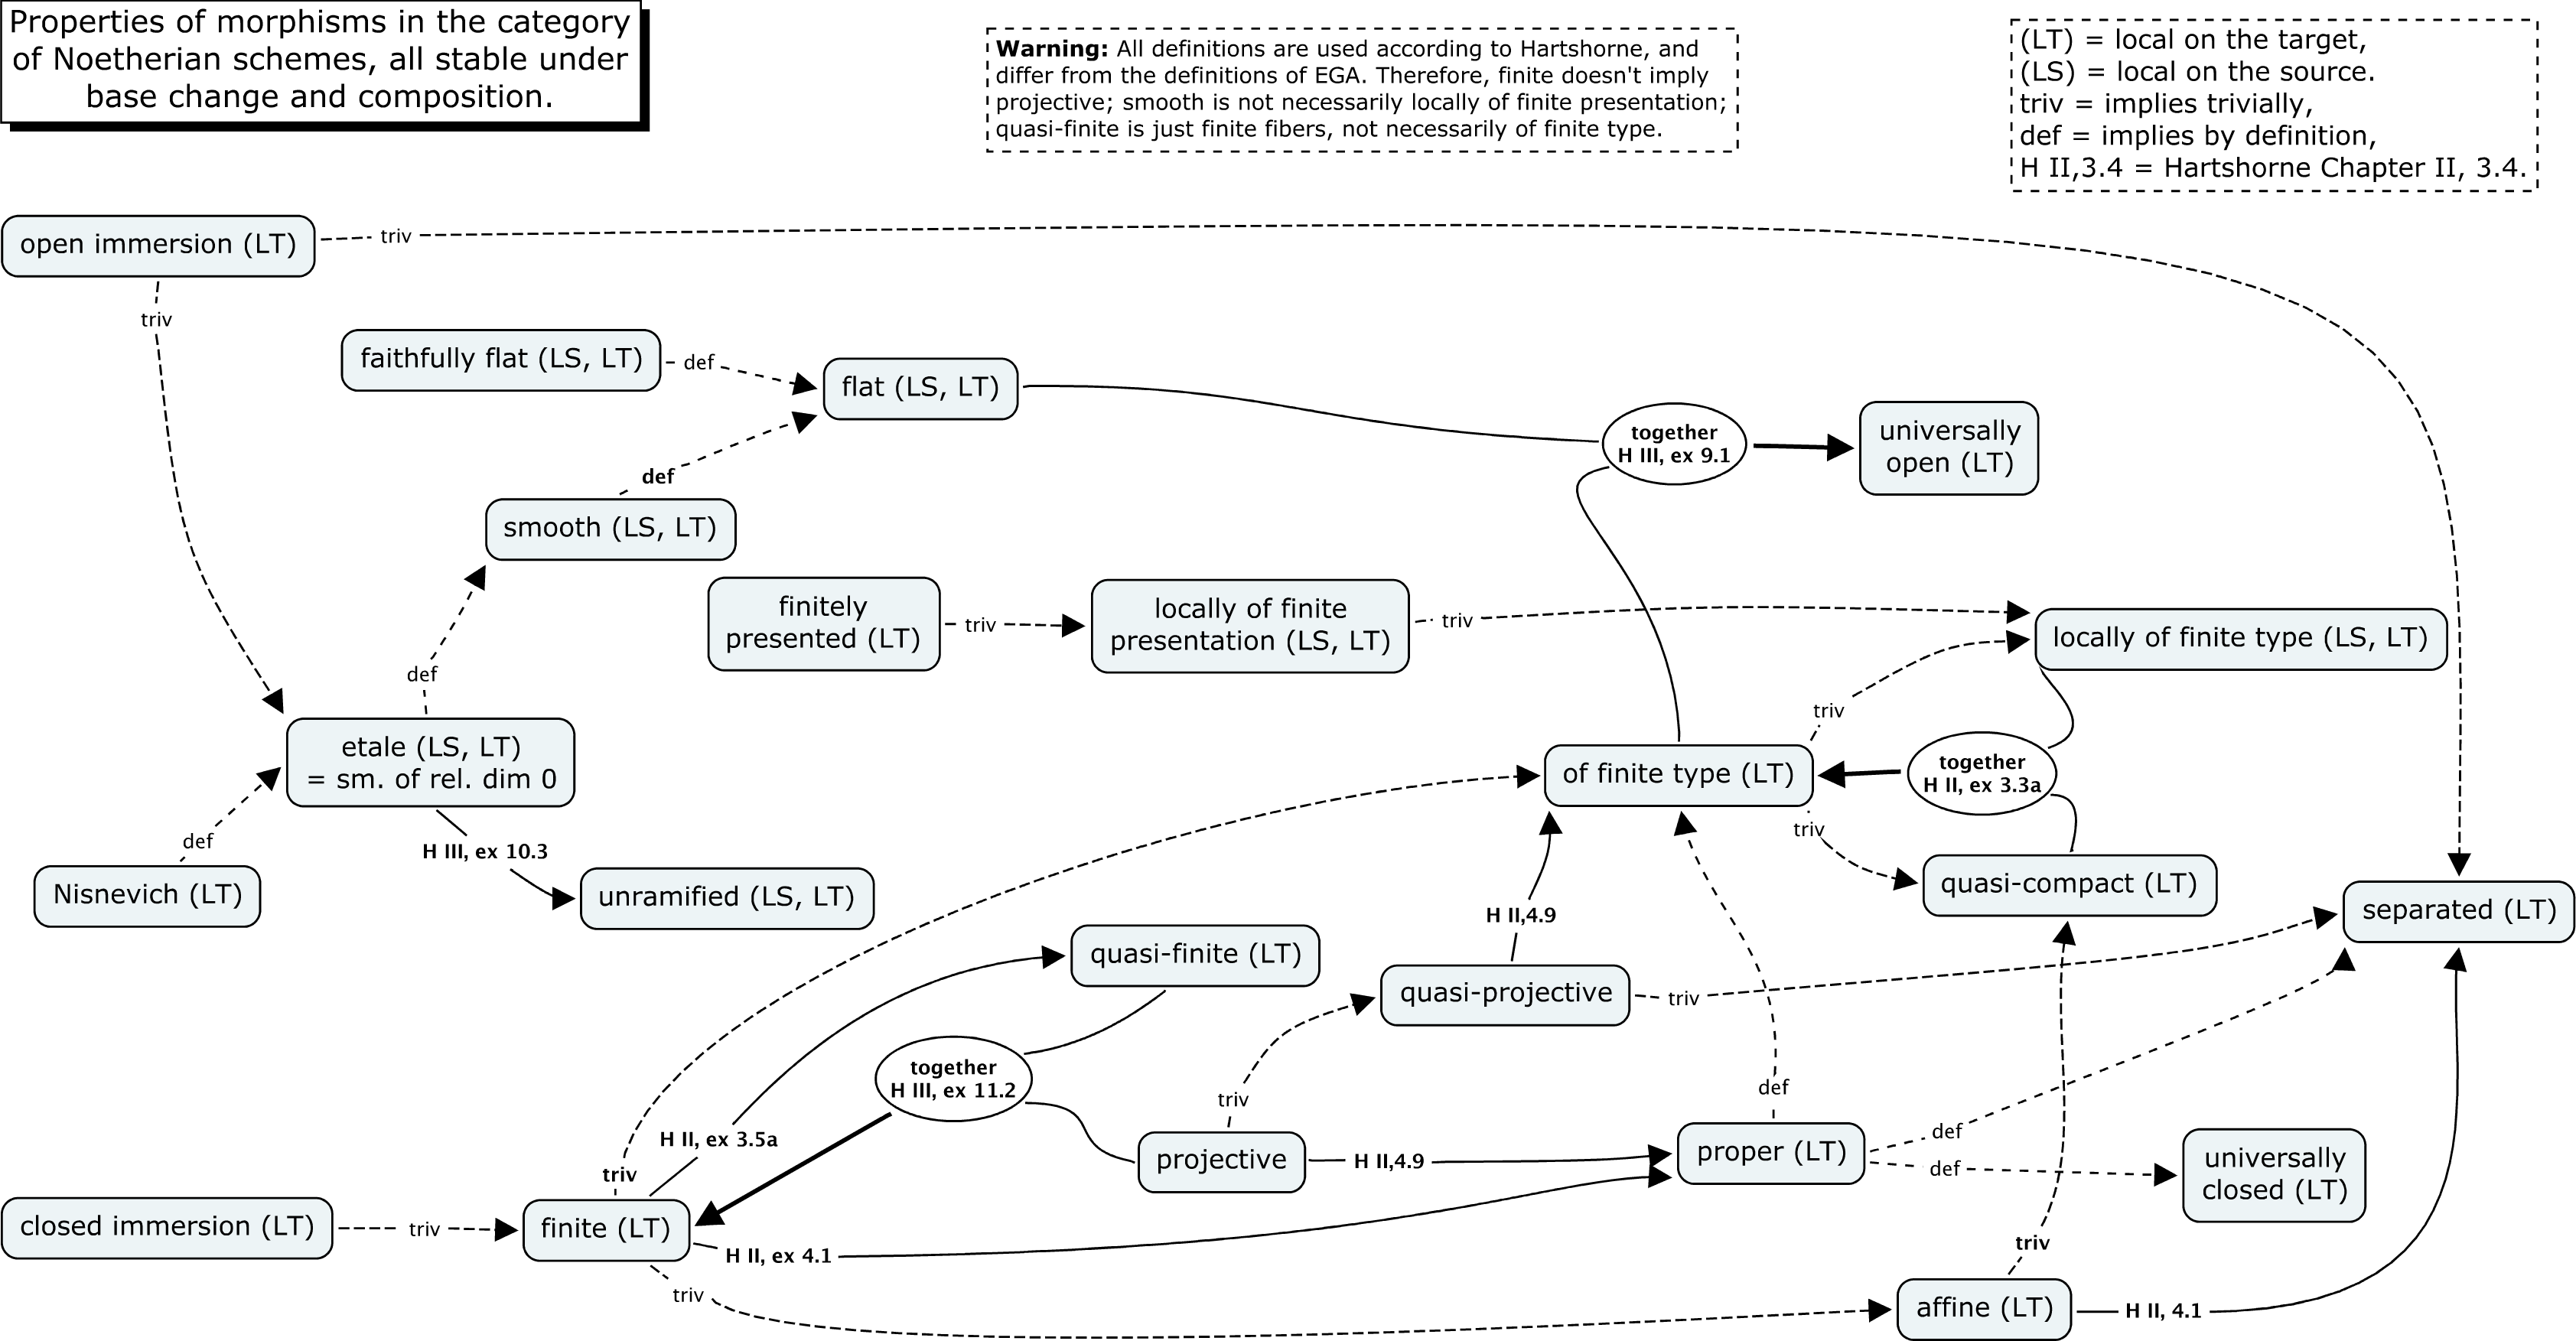
\includegraphics[width=\textwidth]{img/morphisms.png}
\caption{Properties of scheme morphisms. Konrad Voelkel}
\label{fig:Properties of sheme morphims; Konrad Voelkel}
\end{figure}
\end{document}